\documentclass[a4paper]{article}
\usepackage{cmap}
\usepackage{mathtext}
\usepackage{amssymb}
\usepackage{amsmath}
\usepackage[russian]{babel}
\usepackage{indentfirst}
\usepackage[pdftex]{graphicx}
\usepackage{multirow}
\usepackage{mathrsfs}
\usepackage{siunitx}
\usepackage[left=2cm,right=2cm,top=2cm,bottom=2cm]{geometry}
\usepackage{fancyhdr}
\pagestyle{fancy}
\newcommand{\rref}[1]{(\ref{#1})}
\newcommand{\mbf}{\mathbf}
\newcommand{\picref}[1]{рис. \ref{#1}}
\newcommand{\Equip}[3]{
	
	{\bf #1:} $\Delta = \pm #2$ \si{#3}}
\newcommand{\equip}[1]{
	
	{\bf #1}}
\newcommand{\labname}{Петля гистерезиса. Динамический метод} 	% название пиши здесь
\newcommand{\labnum}{3.4.5.}										% номер вводи здесь
\fancyfoot{}
\fancyhead[RE, RO]{\thepage}
\fancyhead[LE, LO]{Лабораторная работа \labnum \space \labname}
\title{Лабораторная работа \labnum \space \labname} % Название работы здесь
\author{Иван Сладков}
\begin{document}
\maketitle
\thispagestyle{empty}
\section{Аннотация}
В данной работе проводится исследование петель гистерезиса различных материалов (феррит, пермаллой, кремнистое железо) в переменных магнитных полях и получение начальной кривой намагничивания.

\section{Теоретические сведения}

Если состояние некоторой системы зависит не только от мгновенных значений внешних параметров, но от истории их изменений, говорят, что в системе имеет место гистерезис. Таким свойством обладает магнитный момент ферромагнетика: $\mathbf{ M = M (H) }$. 

\begin{figure}[tpb]
	\centering
	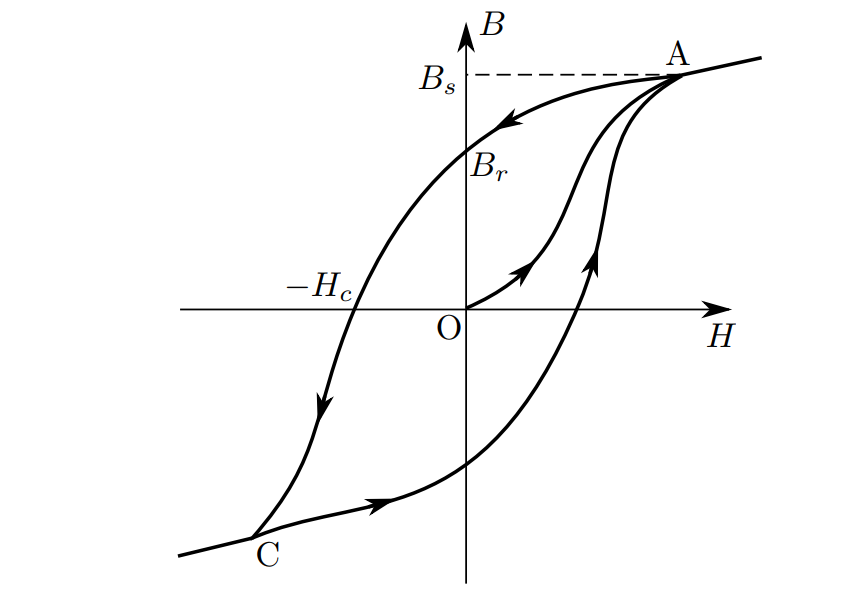
\includegraphics[width=0.8\linewidth]{нач.кривая}
	\caption{Начальная кривая намагничивания и предельная петля гистерезиса}
	\label{fig:кривая-намагничивания}
\end{figure}

Доведём систему до некоторой точки $ A $, лежащей в области насыщения (здесь $ B_s $ — индукция насыщения), и начнём уменьшать напряжённость $ H $. Обратный путь пойдёт не по начальной кривой, а выше неё.

При выключения внешних полей, то есть при достижении $ H = 0 $ в образце сохраняется собственное намагничивание. Соответствующее значение индукции $ B_r $ называют остаточной индукцией.

Значение $ B = 0 $ достигается при отрицательном значении $ H = -H_c $. Величина $ H_c $ называется коэрцитивным полем. В точке $ C $ наступает насыщение для намагничивания в противоположную сторону.
Если теперь попробовать вернуться в точку $ A $, вновь наращивая поле, получим некоторый замкнутый цикл -- предельную петлю гистерезиса (\picref{fig:кривая-намагничивания})). Если в точке $ A $ насыщение не достигается, то аналогичным образом получится цикл меньшей площади.

\subsection{Расчётные формулы}

Из формулы 
\begin{equation*}\label{key}
	\mathscr{E} = - \frac{в \Phi (B)}{d t}
\end{equation*}
получим
\begin{equation}\label{key}
	\left|B\right| = \frac{1}{S N} \int \mathscr{E} d t = \frac{\tau_И}{S N} U_{вых}.
\end{equation}
Последнне соотношение получено, т. к. используем интегрирующую цепочку с постоянной времени $ \tau_И = R_И C_И $.

\section{Оборудование и инструментальные погрешности}

Экспериментальная установка на \picref{fig:установка}. Петля гистерезиса отображается на экране ЭО в масштабе; для уточнения масштаба проводится калибровка.

\begin{figure}[tbp]
	\centering
	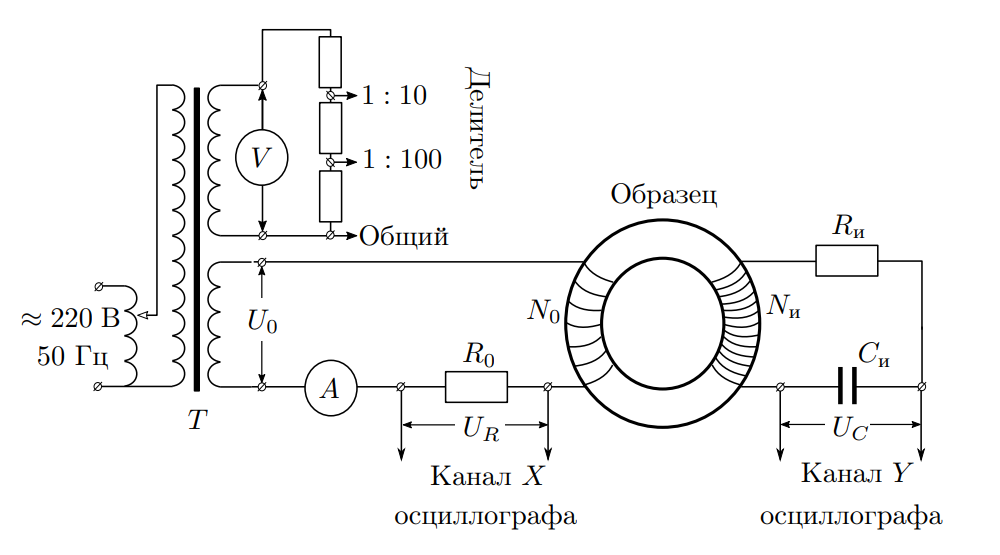
\includegraphics[width=0.8\linewidth]{установка}
	\caption{Установка для исследования петли гистерезиса}
	\label{fig:установка}
\end{figure}

\equip{Автотрансформатор}
\equip{Понижающий трансформатор}
\equip{Интегрирующая цепочка}
\equip{Амперметр}
\equip{Вольтметр}
\equip{Электронный осциллограф (ЭО)}
\equip{Делитель напряжения}
\equip{Тороидальные образцы с двумя обмотками}

Параметры установки соберём в табл. \ref{уст}, \ref{new}.

\begin{table}[]
	\centering
	\begin{tabular}{|l|l|}
		\hline
		$R_0$    & 0.3 Ом \\ \hline
		$R_и$    & 20 кОм \\ \hline
		$C_и$    & 20 мкФ \\ \hline
		$\Omega$ & 50 Гц  \\ \hline
	\end{tabular}
	\caption{Общие параметры}
	\label{уст}
\end{table}

\begin{table}[]
	\centering
	\begin{tabular}{|l|l|l|l|}
		\hline
		& Феррит & Пермаллой & Кремнистое железо \\ \hline
		$N_0$          & 35     & 35        & 35                \\ \hline
		$N_U$          & 400    & 220       & 350               \\ \hline
		$S$, $см^2$    & 3      & 3.8       & 1.2               \\ \hline
		$2\pi R$, $см$ & 25     & 24        & 10                \\ \hline
	\end{tabular}
	\caption{Параметры образцов}
	\label{new}
\end{table}

\section{Результаты измерений и обработка данных}
\emph{Все измерения и расчёты в СИ.}

\subsection{Исследование петли гистерезиса}

Предельные петли для различных образцов изображены на \picref{fig:предельные-кривые}



\begin{figure}[tbp]
	\centering	
	\begin{minipage}{0.33\linewidth}
		\centering
		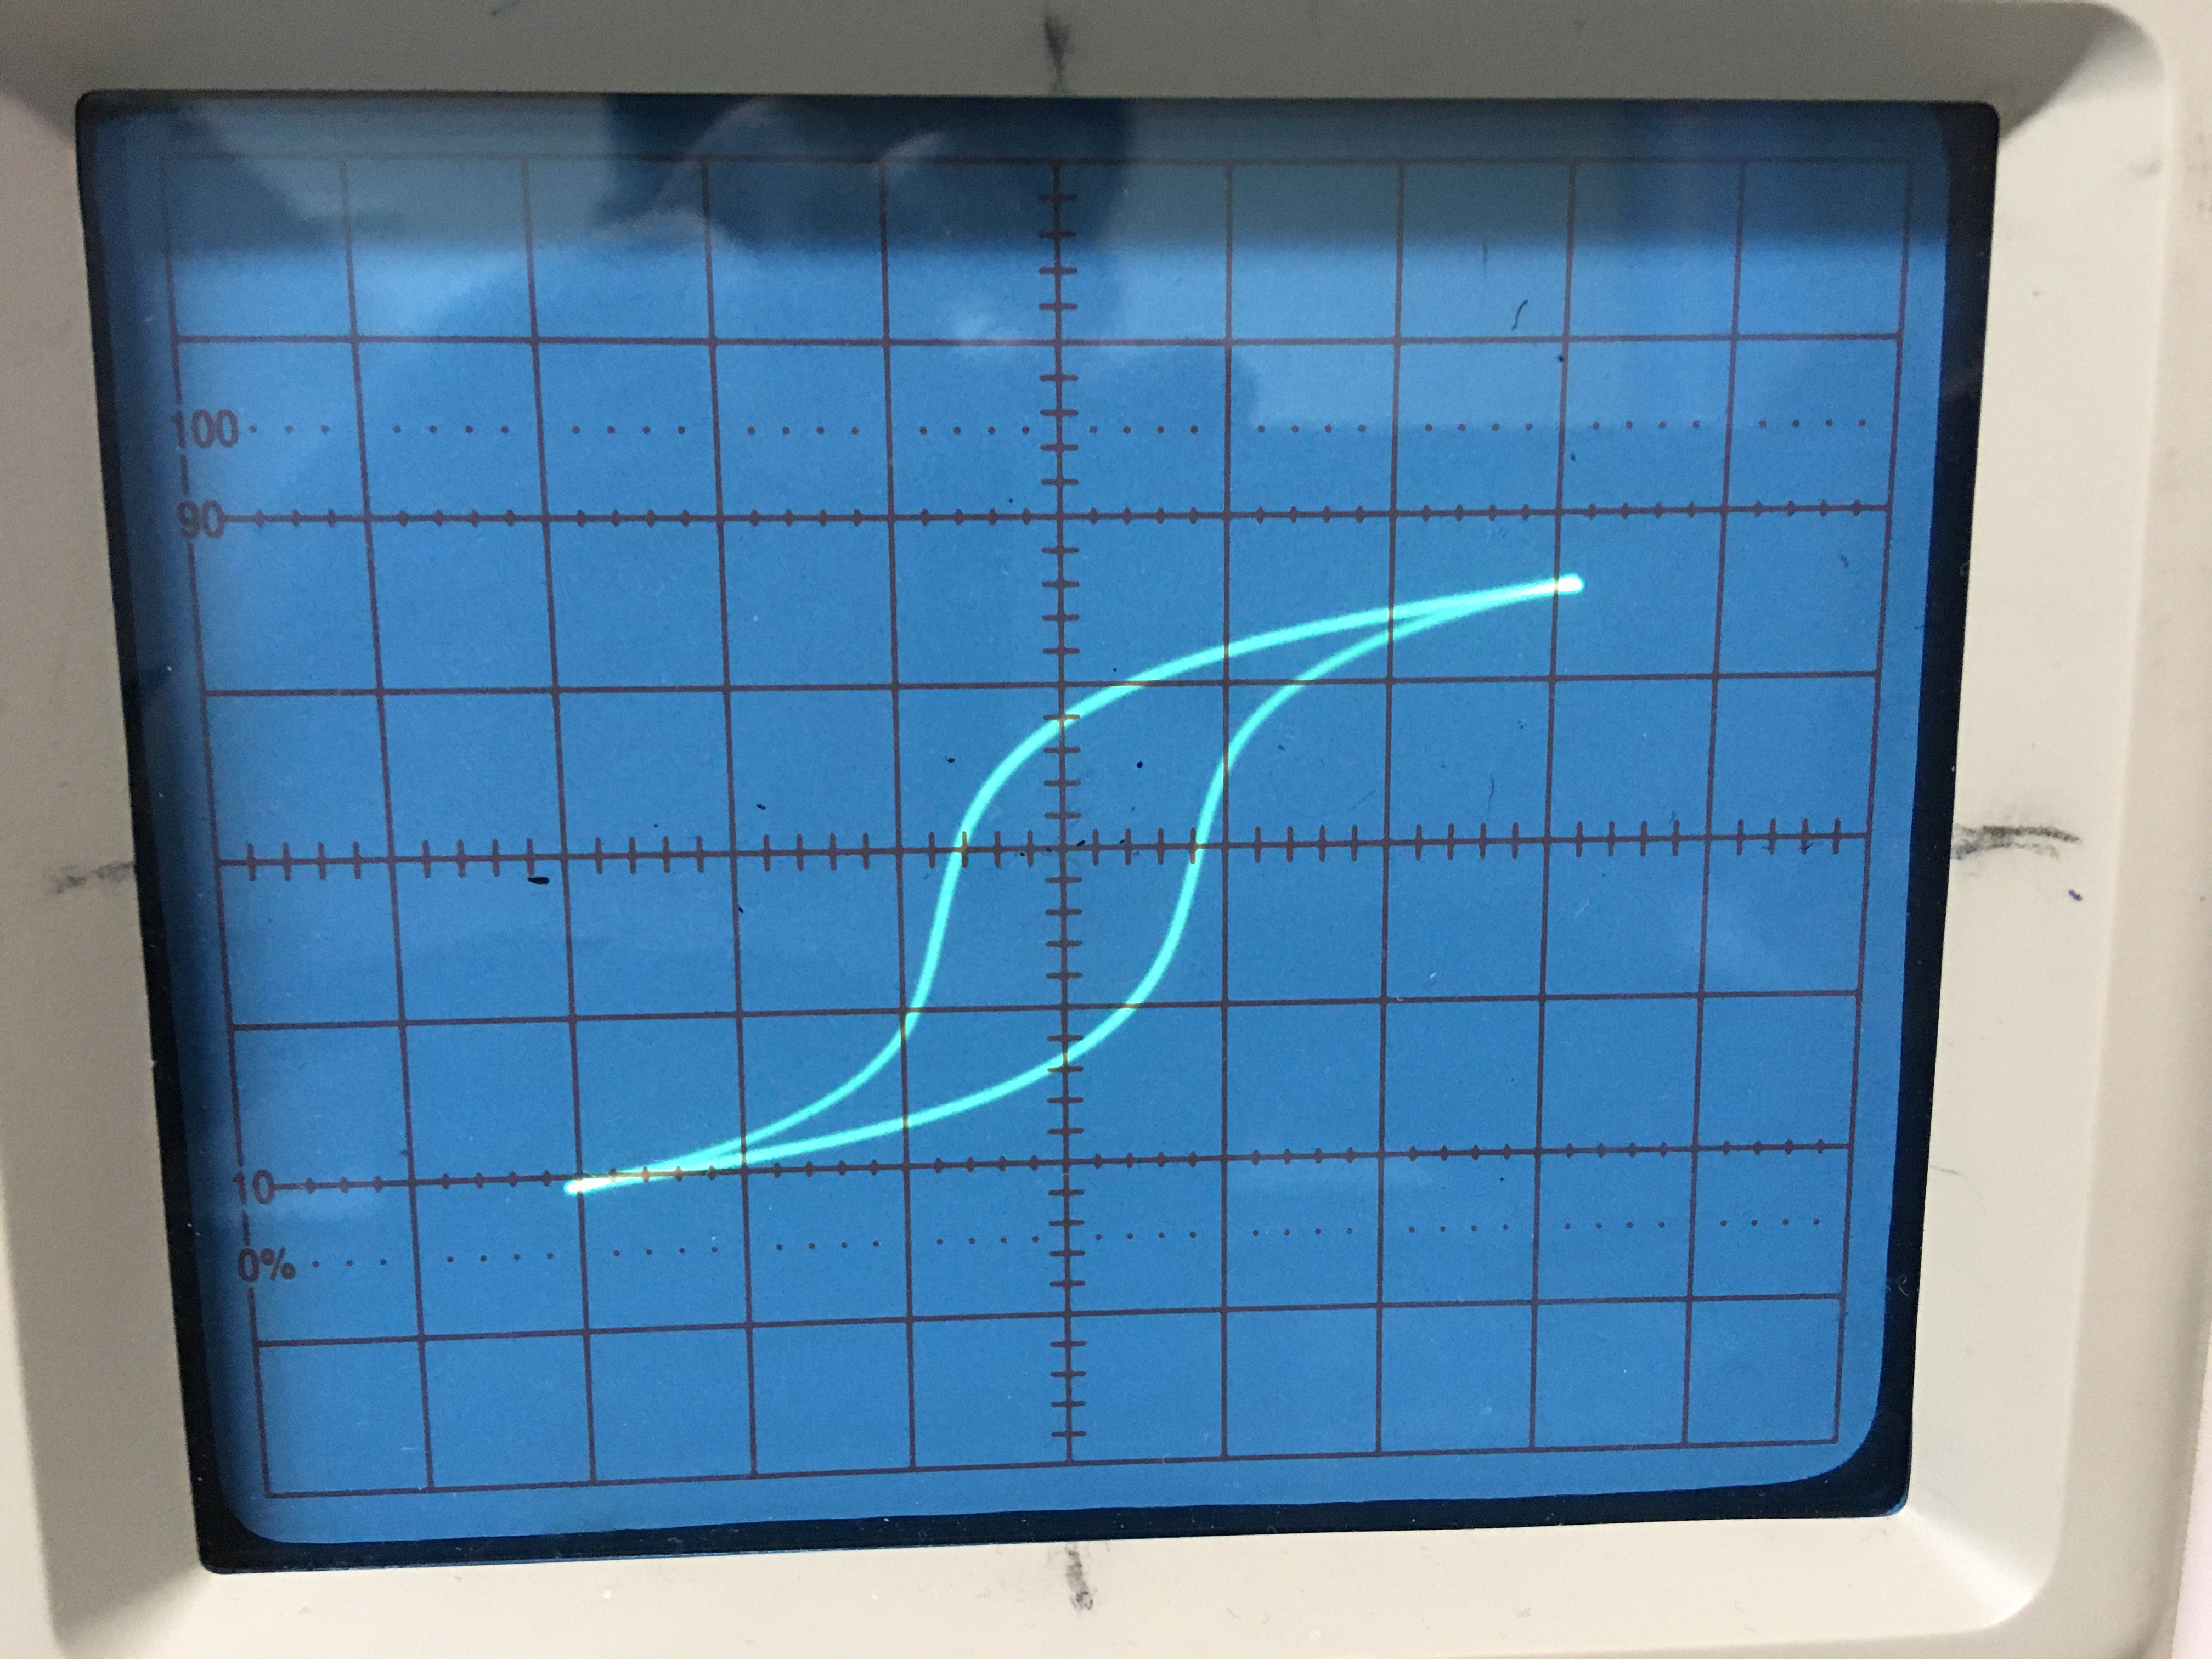
\includegraphics[width=0.9\linewidth]{Результаты/Феррит/IMG_2877}
		Феррит
	\end{minipage}
	\begin{minipage}{0.33\linewidth}
		\centering
		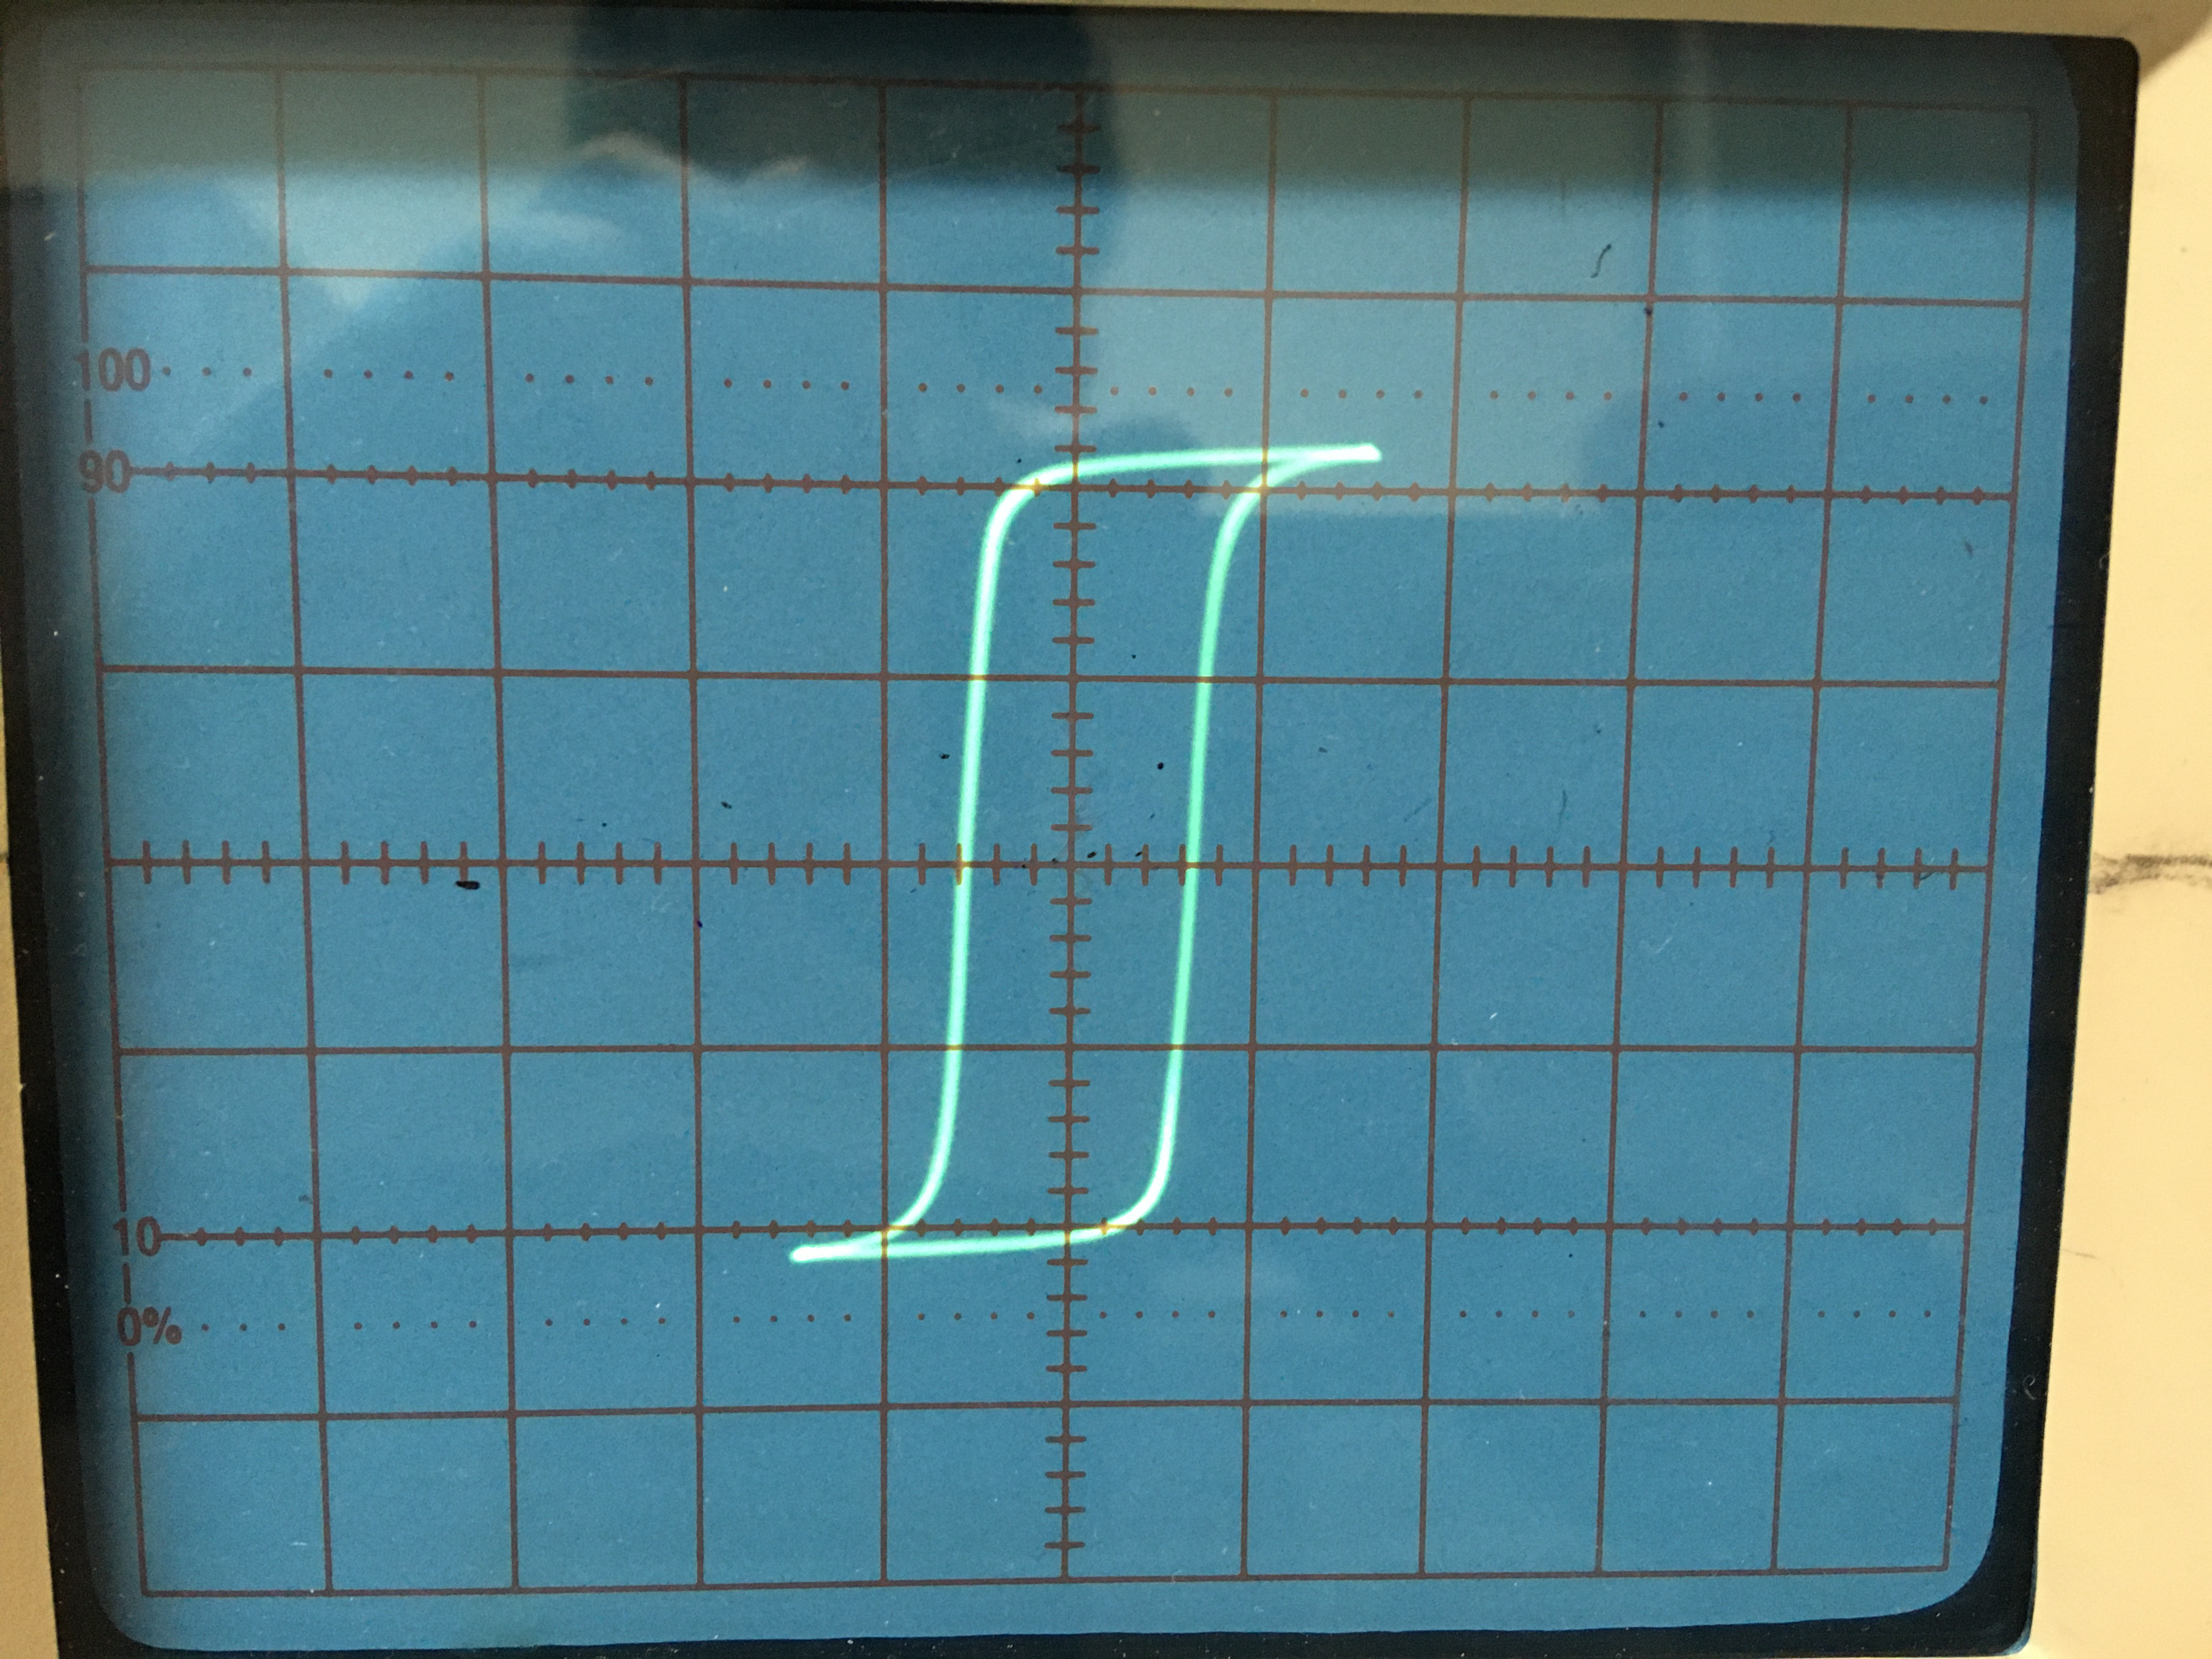
\includegraphics[width=0.9\linewidth]{Результаты/Пермаллой/IMG_2889}
		Пермаллой
	\end{minipage}

	\begin{minipage}{0.33\linewidth}
		\centering
		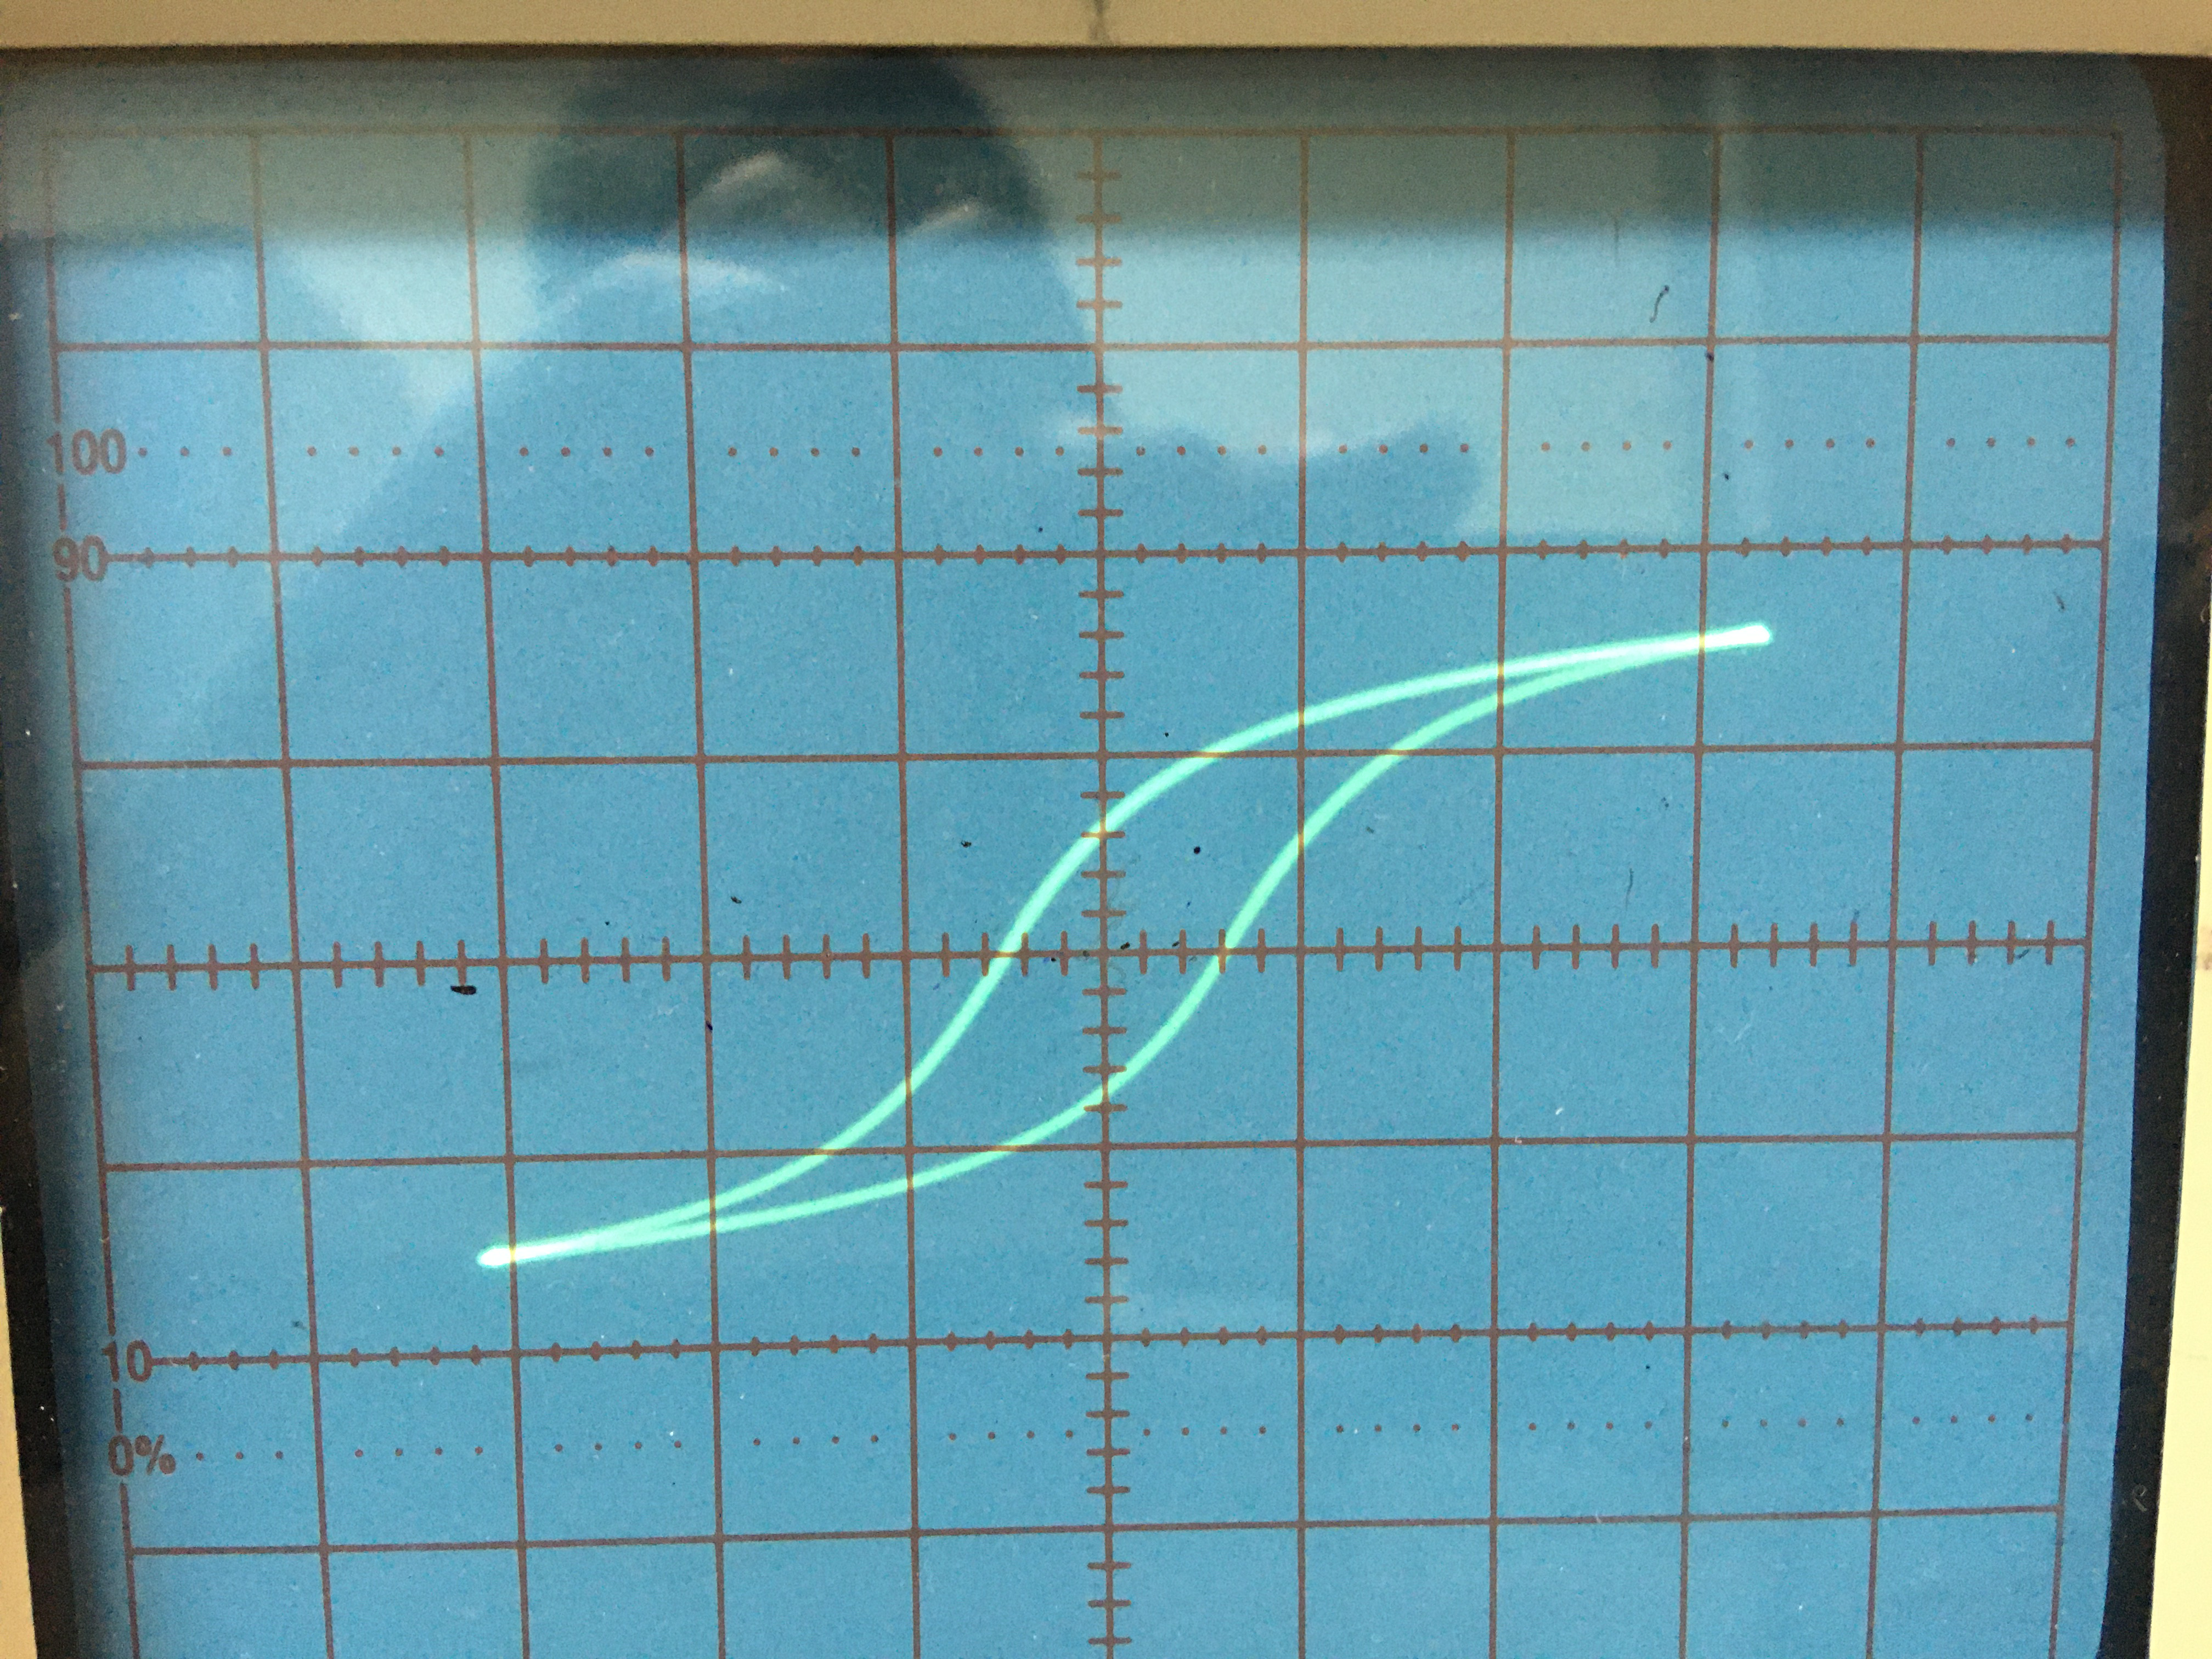
\includegraphics[width=0.9\linewidth]{Результаты/Кремнистое железо/IMG_2903}
		Кремнистое железо
	\end{minipage}

	\label{fig:предельные-кривые}
	\caption{Предельные кривые различных материалов}
\end{figure}

Рассчитаем цену деления.

Для феррита:
\begin{equation*}\label{key}
	h = \frac{K_x N_0}{2 \pi R R_0} = \frac{0.02 * 35}{0.25*0.3} = 9.3 \pm 0.9 \; (А / м) / дел,
\end{equation*}
\begin{equation*}\label{key}
	b = \frac{R_И C_И K_y}{S N_И} = \frac{20000 * 20*10^{-6} * 0.02}{3*10^{-4}*400} = 0.067\pm 0.007 \; Тл / дел.
\end{equation*}

Для пермаллоя:
\begin{equation*}\label{key}
	h = \frac{0.02 * 35}{0.24 * 0.3} = 10\pm 1\; (А / м) / дел,
\end{equation*}
\begin{equation}\label{key}
	b = \frac{20000 * 20*10^{-6} * 0.02}{3.8 * 10^{-4} * 220} = 0.1\pm 0.01\; Тл / дел.
\end{equation}

Для кремнистого железа:
\begin{equation*}\label{key}
	h = \frac{0.1 * 35}{0.1 * 0.3} = 120 \pm 10 \; (А / м) / дел,
\end{equation*}
\begin{equation*}\label{key}
	b = \frac{20000 * 20*10^{-6} * 0.1}{1.2 * 10^{-4} * 350} = 1.0\pm 0.1 \; Тл / дел.
\end{equation*} 

По сделанным фото, учитывая калибровку, построим графики начальных кривых намагничивания.

\begin{figure}[tbp]
	\centering
	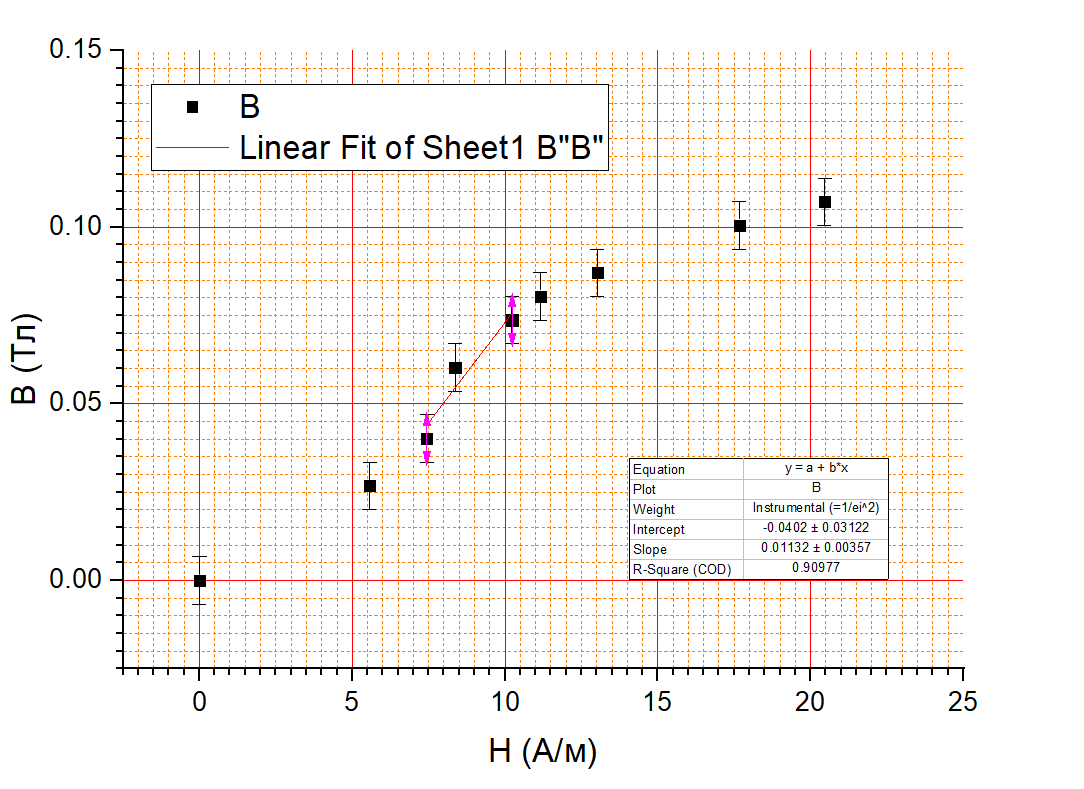
\includegraphics[width=0.8\linewidth]{Феррит}
	\caption{Начальная кривая феррита}
	\label{fig:феррит}
\end{figure}

\begin{figure}[tbp]
	\centering
	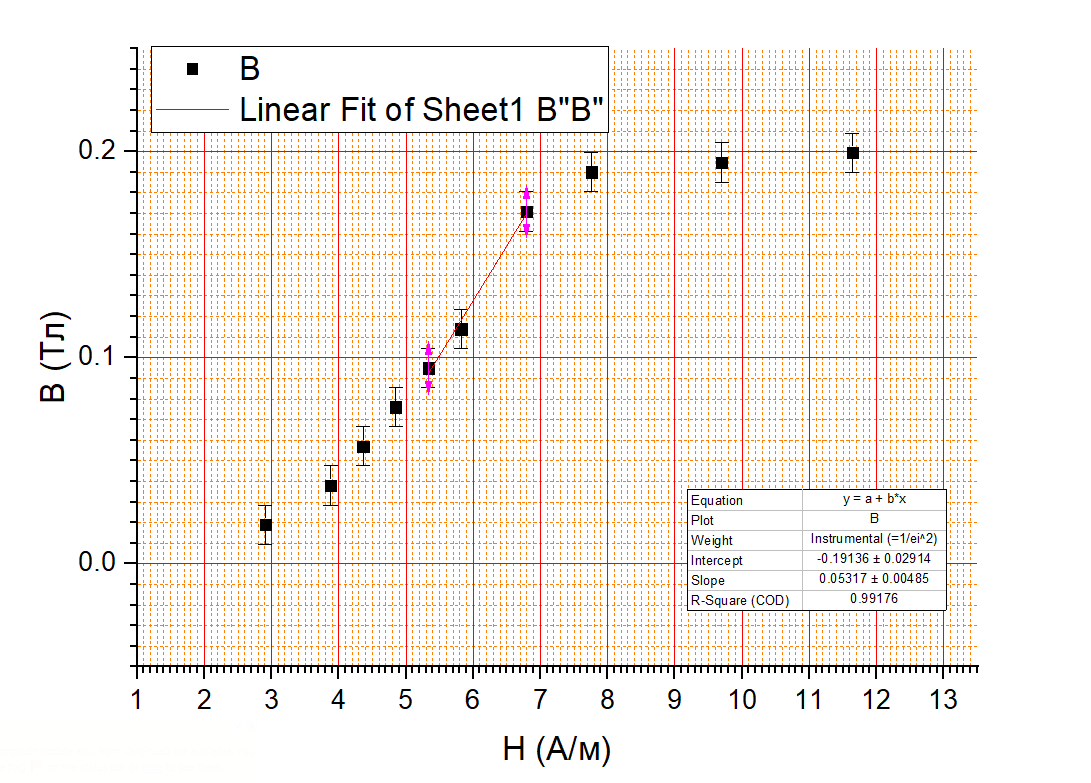
\includegraphics[width=0.8\linewidth]{Пермаллой}
	\caption{Начальная кривая пермаллоя}
	\label{fig:пермаллой}
\end{figure}

\begin{figure}[tbp]
	\centering
	\includegraphics[width=0.8\linewidth]{"Кремнистое железо"}
	\caption{Начальная кривая кремнистого железа}
	\label{fig:железо}
\end{figure}

Далее, найдём индукцию насыщения и коэрцитивную силу.

Для феррита:
\begin{equation*}\label{key}
	H_c = \frac{(2x_c) * h}{2} = 3.1 * 9.3 / 4 = 15.0 \pm 0.1 \; А/м,
\end{equation*}
где $ h $ -- цена деления для $ K_x = 5 \; mV $.
\begin{equation*}\label{key}
	B_s = \frac{(2 y_s) * b}{2} = 2.1 * 0.067 = 0.143 \pm 0.005 \; Тл.
\end{equation*}

Для пермаллоя:
\begin{equation*}\label{key}
	H_c = 3.1 * 9.7 = 30.1 \pm 0.1 \; А / м
\end{equation*}
\begin{equation*}\label{key}
	B_s = 2.9 * 5 * 0.095 = 1.45 \pm 0.03 \; Тл
\end{equation*}

Для кремнистого железа:
\begin{equation*}\label{key}
	H_c = 3 * 116 / 5 = 69.5 \pm 0.2 \; А / м
\end{equation*}
\begin{equation*}\label{key}
	B_s = 3 * 0.95 / 2 = 1.43 \pm 0.03 \; Тл.
\end{equation*}

\subsection{Проверка калибровки по X}

Для $ K_x = 0.1 $ В
\begin{equation*}\label{key}
	m_x = 2 \sqrt{2} R_0 \frac{I_{эф}}{2 x} = 0.098\pm 0.005\; В
\end{equation*}

Для $ K_x = 0.05  $ В:
\begin{equation}\label{key}
	m_x = 2 * \sqrt{2} * 0.3 \frac{0.336}{5.8} = 0.049\pm 0.001\; В
\end{equation}

Для $ K_x = 0.02 $ В:
\begin{equation}\label{key}
	m_x = 2\sqrt{2} * 0.3 * \frac{0.19}{8.2} = 0.0196\pm 0.0002 \; В
\end{equation}

Калибровка по x выполнена с достаточной точностью.

\subsection{Проверка калибровки по Y}

Для $ K_y = 0.1 $ В:
\begin{equation*}\label{key}
	m_y = 2\sqrt{2} U_{эф} / (2y) = 2 \sqrt{2} * 0.138 / 4 = 0.097\pm 0.002 \;B
\end{equation*}

Для $ K_y = 0.05 $ B:
\begin{equation*}\label{key}
	m_y = 2 \sqrt{2} * 0.0814 / 4.8 = 0.48\pm 0.01 \; B
\end{equation*}

Для $ K_y = 0.02 $ B:
\begin{equation*}\label{key}
	m_y = 2 \sqrt{2} * 0.0444 / 6.4 = 0.019\pm 0.003 \; B
\end{equation*}

Калибровка выполнена с достаточной точностью.

\subsection{Оценка $ \mathbf{\tau} $}

$ K_y = 1 $ В/дел.

$ (2y) = 5.6\pm 0.1 $ дел.

$ U_{вх} = 5.60 $ В.

$ U_{вых} = 0.04 $ В.

Тогда:
\begin{equation*}\label{key}
	\tau_{теор} = R C = (20*10^3)*(20*10^{-6}) = 0.4\; c
\end{equation*}
\begin{equation*}\label{key}
	\tau_{эксп} = \frac{U_{вх}}{\Omega U_{вых}} = \frac{5.6}{2 \pi * 50 * 0.04} = 0.44\pm 0.01 \; c
\end{equation*}

$ \tau_{эксп} $ отличается от $ \tau_{теор} $ на 10\%. Это может быть связано, например, с погрешностью при замере $ (2y) $.

\subsection{Оценка погрешностей}

Т. к. в работе присутствует осциллограф, практически все погрешности определяются погрешностью, связанной со снятием показаний по экрану. Т. к. физически невозможно считать показания лучше, чем с точностью 1/10 дел., погрешность $ h $ и $ b $ в пп. 4.1 -- 10\%.

Но при расчёте коэрцитивной силы, погрешность снятия показаний с экрана учтена в $ \sigma_h $, и абсолютная погрешность сохраняется (но только если не меняется масштаб). 

При оценке погрешностей в пп. 4.2 -- 4.4 отн. погр. $ \sigma_{(2 y)}/(2 y) = (10\%)/(2 y) $. Для $ (2 x) $ -- аналогично. Они превалируют над другими инструментальными погрешностями.

\section{Вывод}

Обобщим полученные данные в табл. \ref{tab:my-table}.
% Please add the following required packages to your document preamble:
% \usepackage{multirow}
% Please add the following required packages to your document preamble:
% \usepackage{multirow}
Многие характеристики существенно отличаются от справочных. Скорее всего, это связано с несовершенством метода, а не с низким качеством сплавов (пермаллой НП50, например, прецизионный сплав). По крайней мере, оценочно удалось определить некоторые магнитные параметры данного ряда веществ. Получена примерная кривая намагничивания.

\begin{table}[h]
	\centering
	\begin{tabular}{|l|l|l|l|}
		\hline
		Ампл.                          & Феррит           & Fe-Ni           & Fe-Si          \\ \hline
		\multirow{2}{*}{$H_c, \; А/м$} & $15\pm 0.1$      & $30.1\pm 0.1$   & $69.5\pm 0.2$  \\ \cline{2-4} 
		& $20$             & $11 - 40$       & $100$          \\ \hline
		\multirow{2}{*}{$B_s, Тл$}     & $0.143\pm 0.005$ & $1.45\pm 0.03$  & $1.43\pm 0.03$ \\ \cline{2-4} 
		& $0.15$           & $1.50 - 1.52$   & 2              \\ \hline
		\multirow{2}{*}{$\mu_{диф}$}   & $9010\pm 500$    & $42300\pm 4000$ & $8800\pm 800$  \\ \cline{2-4} 
		& $10000$          & $8000 - 35000$  & $20000$        \\ \hline
	\end{tabular}
	\caption{Сводная таблица магнитных характеристик}
	\label{tab:my-table}
\end{table}

\newpage
\begin{thebibliography}{9}
	\bibitem{Siv} Сивухин Д. В. \emph{Общий курс физики. Том 3 Электричество и магнетизм}, 2004
	\bibitem{kirich} Кириченко Н.А. \emph{Электричество и магнетизм.}, 2011
	\bibitem{max} \emph{Лабораторный практикум по общей физике. В 3 томах. Том 2. Электричество и магнетизм: учебное пособие} под ред. А. В. Максимычева, М. Г. Никулина
\end{thebibliography}
\end{document}